\documentclass[11pt,leqno,a4paper]{report} %fleqn


\usepackage{natbib}
\usepackage{hyperref}
\usepackage{graphicx}
%\bibliographystyle{apacite}
\bibliographystyle{apalike}
\usepackage{booktabs}
\usepackage{epstopdf}
\usepackage{float}
\usepackage{caption}
\usepackage{subcaption}

\usepackage{parskip}


\begin{document}
\begin{titlepage}

\newcommand{\HRule}{\rule{\linewidth}{0.5mm}} % Defines a new command for the horizontal lines, change thickness here

\center % Center everything on the page
 
%----------------------------------------------------------------------------------------
%	HEADING SECTIONS
%----------------------------------------------------------------------------------------

\textsc{\LARGE Radboud University Nijmegen}\\[1.5cm] % Name of your university/college
\textsc{\Large Bachelor Thesis}\\[0.5cm] % Major heading such as course name
\textsc{\large Artificial Intelligence}\\[0.5cm] % Minor heading such as course title

%----------------------------------------------------------------------------------------
%	TITLE SECTION
%----------------------------------------------------------------------------------------

\HRule \\[0.4cm]
{ \huge \bfseries Classifying cognitive load from galvanic skin response time domain features}\\[0.4cm] % Title of your document
\HRule \\[1.5cm]
 
%----------------------------------------------------------------------------------------
%	AUTHOR SECTION
%----------------------------------------------------------------------------------------

\begin{minipage}{0.4\textwidth}
\begin{flushleft} \large
\emph{By:}\\
Guido \textsc{Zuidhof} % Your name
\\\small{guido.zuidhof@student.ru.nl}
\\\small{s4160703}
\end{flushleft}
\end{minipage}
~
\begin{minipage}{0.4\textwidth}
\begin{flushright} \large
\emph{Supervisors:} \\
\small{Dr. }\large Louis \textsc{Vuurpijl}\\ 
\small{Dr. }\large Pashiera \textsc{Barkhuysen}\\
\small{Dr. }\large Ervin \textsc{Poljac}
\end{flushright}
\end{minipage}\\[4cm]

%----------------------------------------------------------------------------------------
%	DATE SECTION
%----------------------------------------------------------------------------------------

{\large \today}\\[3cm] % Date, change the \today to a set date if you want to be precise

%----------------------------------------------------------------------------------------
%	LOGO SECTION
%----------------------------------------------------------------------------------------


\includegraphics[width=300pt]{radlogo.jpg}%\\ % Include a department/university logo - this will require the graphicx package
 
%----------------------------------------------------------------------------------------

\vfill % Fill the rest of the page with whitespace

\end{titlepage}


\tableofcontents 
\thispagestyle{empty}
\addcontentsline



\begin{abstract}
When performing a task, a certain amount of working memory is used. The amount of information a human is trying to process in working memory at any time is known as cognitive load. Biometrics can be used to determine this load. In this thesis galvanic skin response measurements were used to classify the cognitive load of a person. To study this, a pilot experiment was conducted in which every participant performed four tasks with varying difficulty levels, each associated with a certain cognitive load level. An average 4-class classification accuracy of roughly 35\%, and an average 2-class classification accuracy of around 62\% was achieved.

\end{abstract}


\chapter{Introduction}
When performing a task, a certain amount of working memory is used. The amount of information a human is trying to process in working memory at any time is known as the cognitive load of a person \citep{Oviatt2004}. 

With the increasing capabilities of biometric measurement in smartwatches and smartphones it is exciting to see whether these biometric measures can be used to determine the cognitive load of a person. This could allow for dynamic adaptation of an application to best fit the mental state of the user.

This introduction starts with a brief overview of cognitive load theory, followed by an overview of various application areas where knowing the cognitive load of a person can be beneficial. Afterwards the methods of determining the cognitive load of a person is discussed, and the rationale of the chosen method studied in this thesis; a physiological measurement of the galvanic skin response.

\section{Cognitive load}
When processing information, we use working memory. The amount of memory used is not the same for every task. \emph{Cognitive load theory} \citep{Oviatt2004} revolves around the idea that (short-term) working memory is limited, whereas long-term memory is unlimited. 

It is built upon \emph{schema theory}, in which expertise in an area is a function of the acquisition of particular schemata \citep{bartlett1995remembering}. A schema is a mental structure to organise single unit of knowledge. \citep{mcvee2005schema} provides a more complete review of schema theory.

\pagebreak

Cognitive load theory is nearly always studied in the context of learning new schemata. A schema is one element in this working memory, no matter how large it is \citep{mayer2014cambridge}. The idea is that there are ways to reduce cognitive load by utilising long-term memory, and thus having more space in working memory, which would allow for more efficient learning.

Cognitive load theory distinguishes three types of cognitive load, which according to research can each be reduced in specific ways \citep{mayer2002multimedia}:


\paragraph{Extraneous cognitive load}
Influenced by how the material or task is presented. It can be reduced by using worked-out examples, using diagrams, or presenting the material in multiple modalities \citep{mousavi1995reducing}.

\paragraph{Intrinsic cognitive load}
Determined by the complexity of the material at hand. It can be reduced by splitting up the task or building upon former (informal) knowledge.

\paragraph{Germane cognitive load}
The cognitive load associated with the process of building, acquiring and automating new schemas. The greater the space in working memory for this load (by reducing the intrinsic and extraneous cognitive load), the greater the ease of learning.

\section{Applications}
There are many application areas where knowing the cognitive load of a person yields valuable information. Here I will highlight three:

\paragraph{Learning}
Most applications and research regarding cognitive load theory is applied in the context of multimedia learning \citep{brunken2003direct}. The goal in this domain is to find the way to structure and present information to ease learning the most. In other words, to reduce the intrinsic and extraneous cognitive load as much as possible, so that more working memory is left for germane cognitive load. Generally speaking, presenting information in more modalities in multimedia learning tasks decreases the intrinsic and extraneous cognitive load of the task. An example is the use of figures and graphs to visualize information explained in text.

\pagebreak

\paragraph{Usability testing}
Cognitive load measures, and more generally stress and arousal measures, are used by human computer interaction (HCI) developers and researchers to evaluate the usability of software or systems \citep{Jacob2003} \citep{Schmutz2009}.

\citet{Schmutz2009} investigated cognitive load measurement in web applications. Concluded was that cognitive load measures can be used as a \textit{"valuable additional measure of efficiency"}, which strongly correlated to general satisfaction of the user. 

\paragraph{Mental workload}

A universally agreed upon exact definition of mental workload is non-existent, and cognitive load and mental workload are sometimes even used interchangably. 

Here mental workload refers to the amount of human information processing capacity needed for a task, whereas cognitive load refers to the amount of working memory required to perform a task.

The interaction of mental workload and the three types of cognitive load has been studied by \citet{Galy2012269}. Increasing the cognitive load, for instance by increasing the difficulty of the task, was shown to have an additive interaction with mental workload.

It is known that the cognitive load of a person can be used as an indicator for the mental workload of the person. Dynamically using this information to scale up or down the cognitive load of an application can be used to prevent mental overload, which can lead to accidents at work. 
 
This influencing of mental workload can also be used for training purposes, for instance in a game setting. 

%ref naar CFEA / michel?

\section{Determining cognitive load}

There are many approaches to determining cognitive load. The figure below, from \citet{brunken2003direct}, puts the different methods in a matrix based on their objectivity and causal relationship between measurements and cognitive load. Every end of this spectrum has it's benefits and downsides, for instance, subjective methods are a good way to measure the cognitive load associated with any task by having the subject fill out a questionnaire. They are however self-reported measures and thus subjective, which means that the honesty and quality of introspection of subjects may play a role in the results. 

\pagebreak

An example of a (post-event) subjective measurement method is the \emph{NASA Task Load Index (NASA-TLX)} \citep{hart1988development}. This is a questionnaire filled in by the subject after an event where the subject is asked about perceived workload.

On the other end, there are the objective measures, these generally require a more careful design of experiments. The benefit is that they are objective, which means it is not subject to the issues associated with subjective measures described above. In this thesis the indirect, objective method of \emph{physiological measures} is studied. 

\begin{figure}[H]
  \centering   
    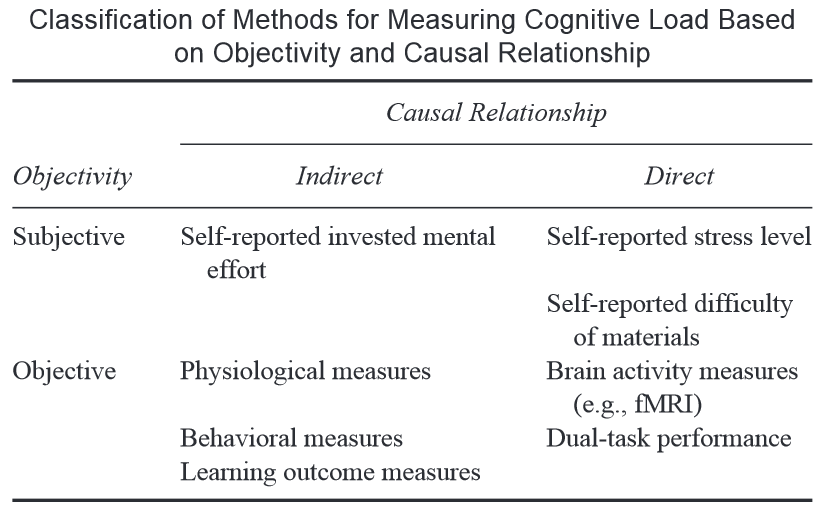
\includegraphics[width=0.84\textwidth]{meas.png}
  \caption{Methods of determining cognitive load. \citep{brunken2003direct}.}
\end{figure}


One of the main benefits of this approach is the objectivity and the possibility of using the cognitive load measurement dynamically, whereas with other objective measures the task has to be completed and the results analyzed.
Downsides of this approach are the possibility of noisy data, sensors may have slight defects and what one measures may be only partially influenced by the cognitive load of a person. Also, the participants have to wear sensors or one has to be in front of a sensor (such as a camera for eye blink rate measurement), which may restrict movement. 

Psychiological measures such as heart rate \citep{hrn}, blink rate \citep{gowrisankaran2012asthenopia}, pupillary dilation \citep{klingner2008measuring}, skin conductance \citep{Nourbakhsh2012} have been shown to correlate with cognitive load. In this thesis skin conductance was the biometric of choice. In the next section I will explain the rationale behind the decision.


\subsection{Galvanic Skin Response}

Galvanic Skin Response (GSR) is an interesting physiological response to measure as sensors are cheap and simple. Also, the subject is not or marginally restricted in movement, allowing for long-term measurement (all day). To this end GSR is the biometric of choice in this explorative study.

Because of these features mobile GSR measurement systems, for instance around the foot \citep{Gravenhorst} are being developed to measure (patients) throughout the day. Also, new devices such as smartwatches are fitted with GSR electrodes increasingly often, which means findings could be applied there. An example would be using GSR data measured by a smart watch to dynamically change an application's presentation of information. For instance, more or less details displayed on the screen depending on the GSR signal.

GSR can be measured in two ways, by measuring conductance (in siemens) or resistance (in ohms). Measuring skin conductance \textit{"bears a simpler more linear relationship to the underlying processes of psychological interest than its repriprocal, SR [skin resistance]"} \citep{lykken1971direct}, therefore any GSR measurement in this thesis is done by measuring skin conductance.

\begin{figure}[H]
  \centering   
    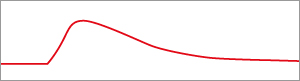
\includegraphics[width=0.9\textwidth]{gsr.jpg}
  \caption{Typical skin conductance response (SCR) \citep{dow_sc_explained_}.}
\end{figure}

Above is a figure showing the typical skin conductance response to a discrete stimulus. Note the response onset, this onset can be up to 4 seconds from the stimulus onset \citep{dow_sc_explained_}. After the peak, an exponential decay is observed.

\pagebreak

\section{State of the art}
Galvanic skin response readings have been studied with regard to cognitive load.

\citet{Shi2007} investigated the possibility of using GSR as an index of cognitive load during the use of unimodal and multimodal versions of the same interface. It has been shown that multimodal interfaces \textit{"support the user in managing cognitive load"} \citep{Oviatt2004}, and thus multimodal interfaces have a lower corresponding cognitive load. 

Shi et al. found that GSR values increase when cognitive load levels increase across all subjects, and conclude that GSR can "serve as an objective indicator of [a] user's cognitive load".

\citet{Nourbakhsh2012} showed that both time and frequency domain features from GSR data significantly correlate with the cognitive load of a person.

In the follow-up research GSR and blink features were used for cognitive load classification \citep{Nourbakhsh2013}. Combining these two featuresets, around 75\% accuracy for binary classification, and 50\% accuracy for four-class classification was achieved. Only GSR features lead to accuracies of around 66\% and 35\% for binary and 4-class classification resepctively.

\citet{library978540} analyzed the mental stress and workload using both galvanic skin response and heart rate variability. The aim was to find the correlation between mental stress and design activities. These activities included designing various objects, such as a house that can easily fly to another place. The results showed that the mean GSR levels were significantly higher during the task compared to the resting state, and the post-test resting state GSR was also significantly higher than the pre-test resting state level.

Novel ways of measuring skin conductance are also studied. \citet{A6945148} used a conductive, flexible polymer foam material to create a sensor that measures the signals from the back of the user. This sensor was easily attached and detached from ordinary clothes, and a correlation to more ordinary GSR sensors (finger electrodes) proved to be high enough to show the feasibility of this new way of measuring GSR.

\pagebreak

\section{Research aim}
The goal of this thesis is to investigate the possibility of determining what the cognitive load of a person is, given GSR measurements. An explorative experiment will be used with different tasks, each of which evokes a different level of cognitive load. From this data a classifier is built, which can classify which task the user was doing based on features derived from GSR, and thus say something about the cognitive load of a person.

The research question reads:

\begin{center}
Can induced cognitive load be classified from galvanic skin response measurements?
\end{center}


\subsection{Organization of this thesis}
In the next chapter I will explain the method with which this research question is answered. Then, in chapter three, the results will be presented, and their implications discussed in the final chapter.

\chapter{Method}

\section{Experiment}
The experiment is mostly based on the arithmetic task experiment conducted by Nourbakhsh et al. \citep{Nourbakhsh2012}. The experiment involves adding up four numbers, displayed one by one, and selecting an answer from three possible answers.

There are four difficulty levels of this task. Difficulty level one involves adding up four binary numbers (1 and 0). Difficulty level two, three and four consist of adding up  four numbers with a length of one, two and three digits respectively.

The subject is first shown an amount of stars corresponding to the difficulty level for 8 seconds, after which the numbers are shown one by one for 4 seconds. Three answers are then presented on the screen, of which one is correct. The subject subsequently selects the correct answer using a standard computer mouse. There was no time limit for selecting an answer.

In \citet{Nourbakhsh2013} these tasks were shown to have significant difference in subjective ratings of task difficulty levels, as well as a siginificant difference in response time of different task levels. This implies that these designed tasks manipulate cognitive load effectively.


\subsection{Apparatus}
The task was displayed on a 15.6" laptop screen, and input was given using a standard computer mouse.
Two galvanic skin response sensors were used in this experiment. The participants wore both sensors at the same time on the left arm. Below, the two sensors are briefly discussed.

\begin{figure}[H]
\hspace*{-.1\textwidth}        \centering
        \begin{subfigure}[b]{0.6\textwidth}
                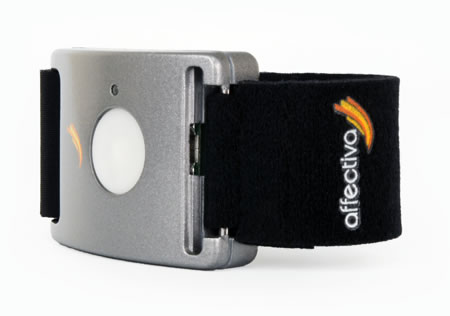
\includegraphics[width=\textwidth]{affectiva.jpg}
                \caption{Affectiva Q Sensor}
                \label{fig:aff}
        \end{subfigure}%
        ~ 
        \begin{subfigure}[b]{0.6\textwidth}
                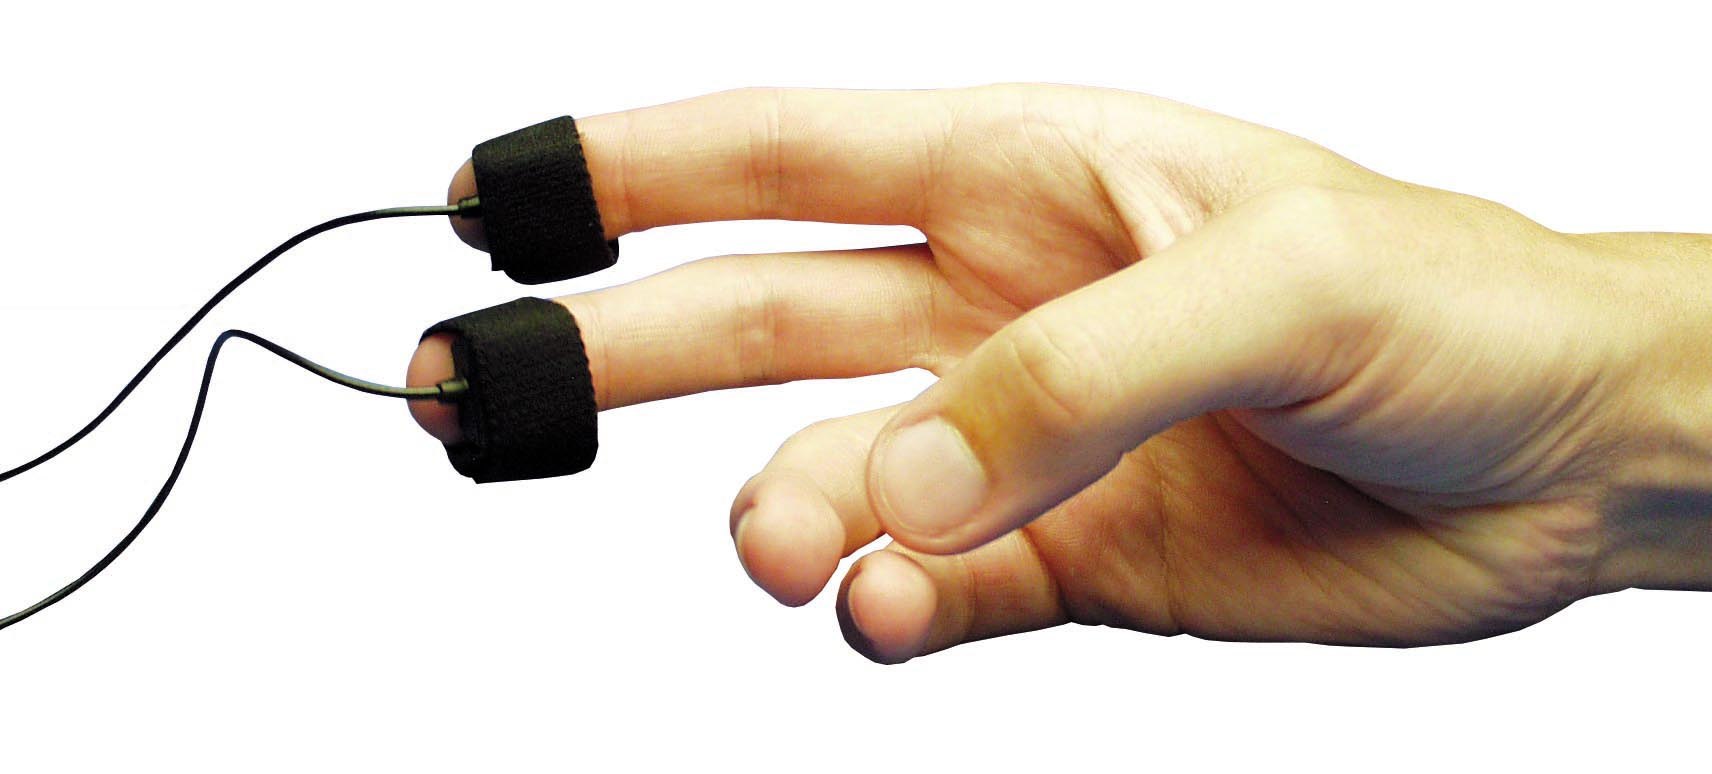
\includegraphics[width=\textwidth]{bioelec.jpg}
                \caption{BIOPAC MP30 finger electrodes}
                \label{fig:bio}
        \end{subfigure}
        \caption{Sensors used in the experiment}\label{fig:animals}
\end{figure}


\paragraph{Affectiva Q Sensor}
This sensor is embedded in a wrist band, it uses a dry electrode. The sensor side of the wrist was placed on the bottom of the wrist. The sampling rate of this sensor was set to 32 samples per second. This is the highest possible sampling rate setting of this device.

\paragraph{BIOPAC MP30}
The BIOPAC MP30 was used in conjunction with finger GSR sensors. This sensor wraps around two fingers, in this experiment the index and ring finger. It uses gel electrodes, Grass EC33 Electrode Paste was used for this purpose.

The sampling rate was set to 1000 samples per second. This is an arbitrarily chosen high sampling rate, much higher than the frequencies at which \citet{Nourbakhsh2012} found significant differences in the power spectrum between the different tasks.

\subsection{Participants}
Six participants took part in this experiment, five male and one female. Their age ranged between 19 and 25 at the time of the experiment. They were not compensated for their participation.


\subsection{Experimental Design}
The task consisted of 8 arithmetic tasks, with 4 difficulty levels. Two tasks of every difficulty level were completed by the participants, in a random order. 

A single task consisted of adding up four numbers, and selecting an answer from three options. The numbers were shown one by one, for four seconds. Before a task started, a number of stars was shown equal to the difficulty level, for eight seconds. The tasks followed each other without breaks. There was no time limit for selecting the answer and there was no feedback whether the selected answer was correct.

\begin{figure}[H]
  \centering
 	\hspace*{-.25\textwidth}   
 	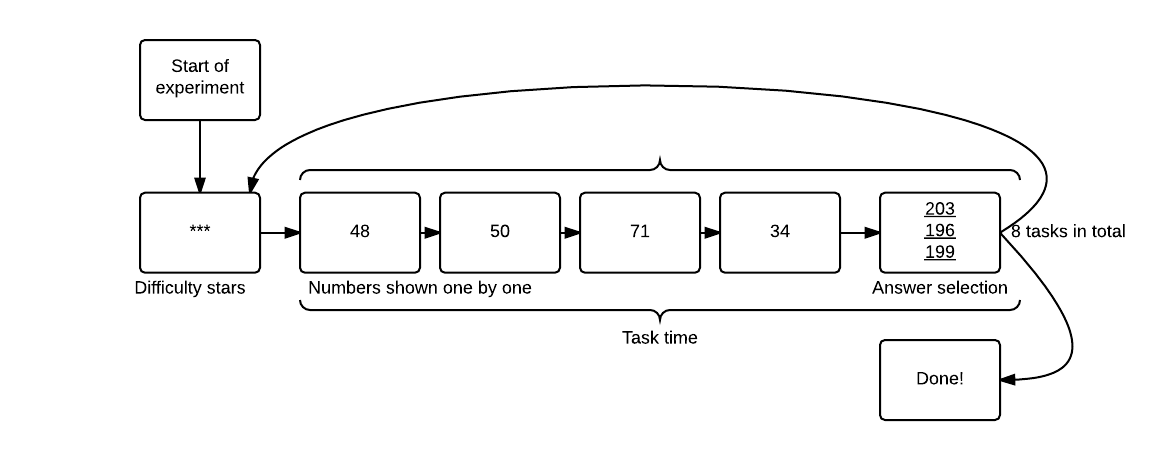
\includegraphics[width=1.5\textwidth]{experiment.png}
  \caption{Experiment structure}
\end{figure}

\subsection{Procedure}
The participants were seated in front of a laptop and the experimenter explained the task. Then the sensors were applied to the left hand and wrist. The participant was then instructed to place the left hand on the table in front of him/her and not to move it, in order to prevent possible motion artifacts which have earlier been shown to influence GSR readings \citep{motionart}.

\pagebreak

\section{Analysis}

\subsection{Affectiva Q Sensor Data}
The data gathered from the Affectiva Q Sensor proved to be unusable. In most participants no proper skin contact seemed to have been made during the full experiment. Dry GSR sensors need some sweat to ensure a good connection with both electrodes. Given the short experiment duration (a few minutes) this connection was possibly never established.

%In hindsight the participants could have worn the device longer before the first task started, or they could have been asked to perform some light exercise. 

Therefore, any data discussed from here on is solely that which has been collected using the BIOPAC MP30 and it's finger electrodes.


\subsection{Preprocessing}
All data files were preprocessed using custom scripts written in \emph{MATLAB (The MathWorks, Inc.)}. The collected data contained a DC current, which was smoothed by filtering and resampling to 100 samples per second using a Savitzky-Golay filter \citep{savitzky1964smoothing}. 

The data per subject was then cut into separate frames, the tasks. A task (slice of data) runs from the time that the first number is shown, to the time that an answer is given. These tasks were then smoothed one last time, to get rid of a small remaining amount of DC noise. This was again done using a Savitzky-Golay filter.

The data was then normalized per subject over all datapoints in all tasks. This was done by dividing every data point of the subject by the average of the subject over all tasks. 

Let the average over all tasks:


\[
AverageGSR(s) = \frac 
{\sum_{q \in Q_s}\sum_{t \in T_q} GSR(s,q,t)}
{ \sum_{q \in Q_s} \left\vert{T_q}\right\vert }
\]

With $s$ a given subject, $Q_s$ a set of all tasks performed by $s$, and $T_q$ the set of all measurements in task $q$, and $GSR(s,q,t)$ be the GSR datapoint of subject s, task q at time t.

\pagebreak

The normalised GSR is then given by:

\[
NormGSR(s,q,t) = \frac{GSR(s,q,t)}{AverageGSR(s)}
\]

Note that the normalization is done by dividing by the average of the subject over all tasks, and not by simply transforming all measurements to be between 0 and 1. What (original) GSR value would become 1 and 0 would then be quite arbitrary per subject, and not all subjects would be on the same scale, as outliers can totally influence this range.



This normalised GSR was then cut into the specific tasks.

\subsection{Transformation}
From the measurements from every task certain time domain features were extracted. 

The extracted features:

\begin{itemize}

\item Average over all points in the task.
\item Accumulative of all points in the task.
\item Standard deviation of all points in the task.
\item Difference between first and last point of the task.
\item Peaks with varying tresholds of what a peak is.
\end{itemize}

Below I will elaborate how these features were calculated from the data. In these formula's $s$ is a subject, $q$ is a task and $T_q$ are all the measurements (datapoints) associated with task $q$.

\paragraph{Average}

\[
AvgTaskGSR(s,q) = \frac { \sum_{t \in T_q} NormGSR(s,q,t) }
{\left\vert{T_q}\right\vert }
\]

\paragraph{Accumulative}

\[
AccTaskGSR(s,q) =  \sum_{t \in T_q} NormGSR(s,q,t)
\]

\paragraph{Standard deviation}

\[
StdDevTaskGSR(s,q) = \sqrt {\frac{1}{\left\vert{T_q}\right\vert}   \sum_{t \in T_q} (NormGSR(s,q,t) - AvgTaskGSR(s,q))^2 }
\]

\paragraph{Difference}

\[
DiffTaskGSR(s,q) = NormGSR(s,q, t_{\left\vert{T_q}\right\vert}) - NormGSR(s,q, t_1)
\]
where $t_1$ is the first measurement in $T_q$, and $t_{\left\vert{T_q}\right\vert}$ the last measurement of the task.

\paragraph{Peaks}
For peak detection the \emph{PeakFinder} script \citep{yoder}, found in the \emph{Matlab Central File Exchange} was used under BSD License. This script finds local maxima or minima, even in noisy signals, and can be supplied with a treshold that determines what classifies as a peak.

This script was called with four different threshold levels, given by

\[
Threshold(s,q,k) = \frac 
{\max_{t \in T_q} NormGSR(s,q,t) - \min_{t \in T_q} NormGSR(s,q,t)} 
{(2k)^2}
\]

with $k \in \{1,2,3,4\}$.


\subsection{Data mining}

The extracted features were then fed into \emph{Weka 3} \citep{weka}, which is data mining software in Java. 


Three of the most commonly used classification algorithms were used \citep{small}. Namely a Bayesian classification algorithm (\emph{Na\"iveBayes}, which is an implementation based on \citep{john1995estimating}), a support vector machine (SVM) classification algorithm (\emph{LibSVM}) \citep{libsvm}, with SVM model type C-SVC and a radial basis kernel type, and a neural network classifier (\emph{MultilayerPerceptron}, with 8 hidden layers). 

Two classifiers  were trained with each algorithm, one for 4-class classification, and one for 2-class (binary) classification (with task difficulty 1 and 2 combined, and 3 and 4 combined).


\chapter{Results}

\section{Gathered data}

Below in figure 3.1 the raw data is shown from one of the subject over the course of the whole experiment (including some trailing seconds of disconnecting the measurement device). In figure 3.2 this data has been filtered using the first Savitzky-Golay filter.

%Raw and filtered data of full experiment figure

\begin{figure}[H]
  \centering
    \hspace*{-.25\textwidth}   
    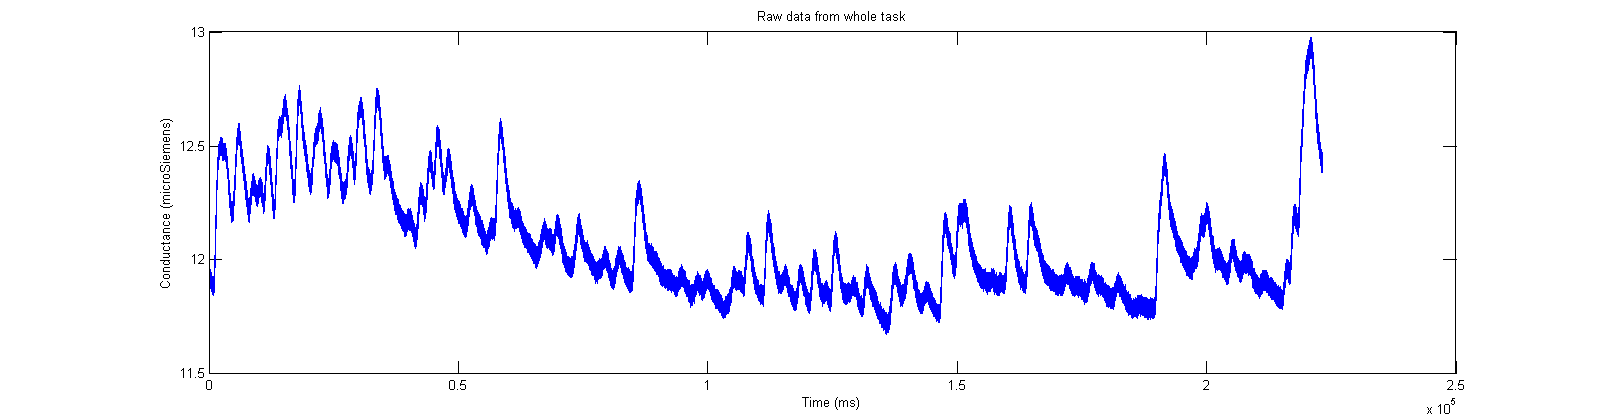
\includegraphics[width=1.5\textwidth]{measurements/raw.png}
  \caption{Raw data from a single participant.}
\end{figure}

\begin{figure}[H]
  \centering
 	\hspace*{-.25\textwidth}   
 	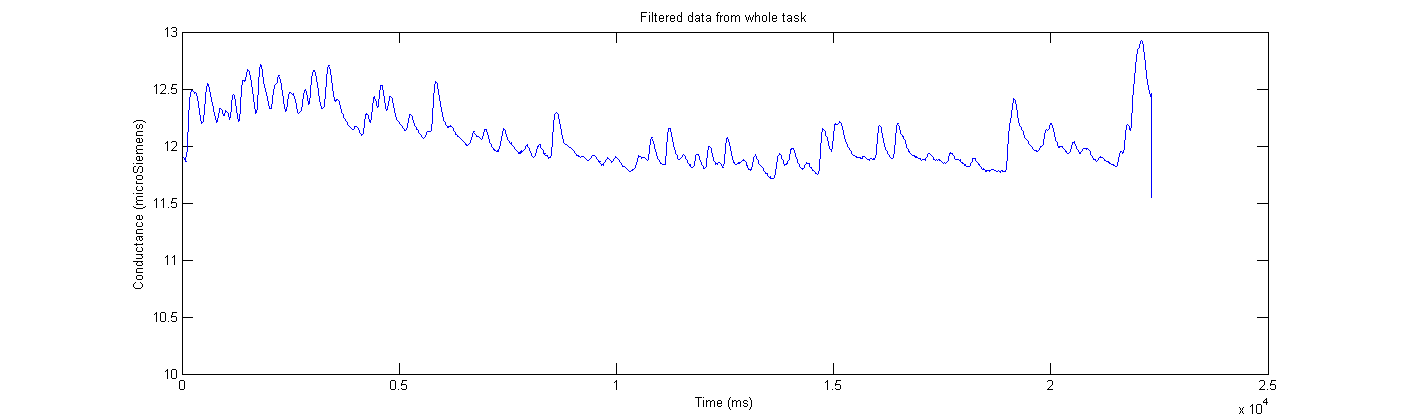
\includegraphics[width=1.5\textwidth]{measurements/filtered.png}
  \caption{Data from a single participant after Savitzky-Golay filter.}
\end{figure}

A typical task's data is shown in figure 3.3a, this is a slice of the data plotted in figure 3.2. In 3.3b this data has been normalized as described in the previous chapter, as well as filtered using a Savitzky-Golay filter to smooth over any remaining noise.

% Single task figure

\begin{figure}[h!]
\hspace*{-.2\textwidth}        \centering
        \begin{subfigure}[b]{0.7\textwidth}
                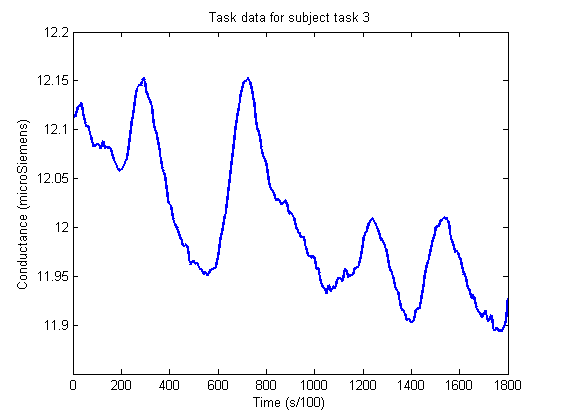
\includegraphics[width=\textwidth]{measurements/singletaskunnormal.png}
                \caption{unnormalized}
                \label{fig:singleunnormal}
        \end{subfigure}%
        ~ %add desired spacing between images, e. g. ~, \quad, \qquad, \hfill etc.
          %(or a blank line to force the subfigure onto a new line)
        \begin{subfigure}[b]{0.7\textwidth}
                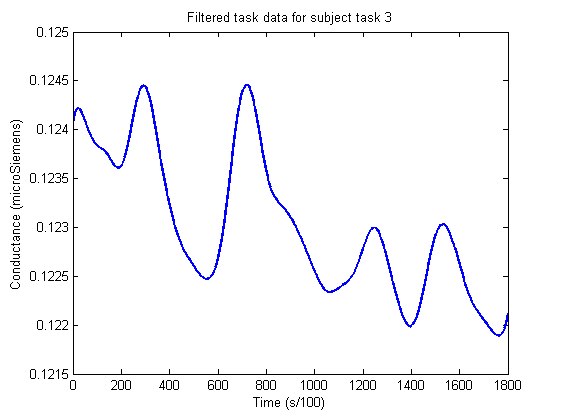
\includegraphics[width=\textwidth]{measurements/singletaskfilt.png}
                \caption{filtered and normalized}
                \label{fig:singlefiltered}
        \end{subfigure}
        \caption{Task 3 (difficulty 2) of subject 2}\label{fig:animals}
\end{figure}

In the appendix of this thesis there are several visualizations of characteristics of the processed gathered data.

\pagebreak




\section{Classification accuracy}
\begin{table}[h]
\caption {Classification accuracy} 
\center
\begin{tabular}{@{}lrr@{}}
\toprule
Classification Algorithm & \multicolumn{1}{l}{2-Class Classification} & \multicolumn{1}{l}{4-Class Classification} \\ \midrule
NaiveBayes               & 62.5\%                                     & 35.4\%                                     \\
LibSVM                   & 68.8\%                                     & 22.9\%                                     \\
MultilayerPerceptron     & 56.3\%                                     & 41.7\%                                     \\ \bottomrule
\end{tabular}
\end{table}

The performance of each predictive model was estimated using 10 fold cross-validation. The percentages in the table are the percentage of correctly classified task difficulties by the predictive model.

\pagebreak

\section{Confusion matrices}
% Confusion matrix NaiveBayes

\begin{table}[h]
\caption {NaiveBayes confusion matrix} 
\center
\begin{tabular}{ccccl}
\multicolumn{1}{l}{1} & \multicolumn{1}{l}{2} & \multicolumn{1}{l}{3} & \multicolumn{1}{l}{4} & \small{\textless- Classified as difficulty} \\ \cline{1-4}
1                          & 7                          & 1                          & \multicolumn{1}{c|}{3}     & Difficulty 1                    \\
3                          & 7                          & 0                          & \multicolumn{1}{c|}{2}     & Difficulty 2                    \\
2                          & 4                          & 2                          & \multicolumn{1}{c|}{4}     & Difficulty 3                    \\
2                          & 2                          & 1                          & \multicolumn{1}{c|}{7}     & Difficulty 4                   
\end{tabular}
\end{table}



% Confusion matrix LibSVM

\begin{table}[h]
\caption {LibSVM confusion matrix} 
\center
\begin{tabular}{ccccl}
\multicolumn{1}{l}{1} & \multicolumn{1}{l}{2} & \multicolumn{1}{l}{3} & \multicolumn{1}{l}{4} & \small{\textless- Classified as difficulty} \\ \cline{1-4}
1                          & 5                          & 6                          & \multicolumn{1}{c|}{0}     & Difficulty 1                    \\
5                          & 3                          & 3                          & \multicolumn{1}{c|}{1}     & Difficulty 2                    \\
3                          & 1                          & 5                          & \multicolumn{1}{c|}{3}     & Difficulty 3                    \\
5                          & 0                          & 5                          & \multicolumn{1}{c|}{2}     & Difficulty 4                   
\end{tabular}
\end{table}

% Confusion matrix MultilayerPerceptron

\begin{table}[h]
\caption {MultilayerPerceptron confusion matrix} 
\center
\begin{tabular}{ccccl}
\multicolumn{1}{l}{1} & \multicolumn{1}{l}{2} & \multicolumn{1}{l}{3} & \multicolumn{1}{l}{4} & \small{\textless- Classified as difficulty} \\ \cline{1-4}
3                          & 4                          & 3                          & \multicolumn{1}{c|}{2}     & Difficulty 1                    \\
3                          & 5                          & 2                          & \multicolumn{1}{c|}{2}     & Difficulty 2                    \\
2                          & 3                          & 6                          & \multicolumn{1}{c|}{1}     & Difficulty 3                    \\
2                          & 1                          & 3                          & \multicolumn{1}{c|}{6}     & Difficulty 4                   
\end{tabular}
\end{table}

These confusion matrices visualize the performance of the classification algorithm. From a confusion matrix one can see how often a class (difficulty of task) is predicted as another class. The correctly classified instances are found on the diagonal (top-left to bottom-right).





\chapter{Discussion}

To rehash, the research question of this thesis reads \emph{Can induced cognitive load be classified from galvanic skin response measurements?}. In this section I will discuss this question with the results from this experiment.

\section{Interpretation}

The results show that the classification accuracy of the classifiers is better than chance dictates for two out of three used classification algorithms, however not much. The binary classification results were more accurate, where every classifier performs better than chance.
These classification rates are slightly lower than those reported by \citet{Nourbakhsh2013} in a similar experiment, which may be due to the smaller dataset.

When considering the confusion matrices of the 4-class classification it can be noted that the task most often classified as having a wrong difficulty level was task 1, which was more often classified as difficulty 2 and 3 than 1. In fact, it has only been classified correct once out of twelve entries in the NaiveBayes and LibSVM model, and a mere three times in the MultilayerPerceptron model. Perhaps this task was too easy and caused participants to become distracted.

There are many possible explanations why this classification accuracy is not greater. The first explanation is that from just GSR data, it simply can not be classified any better. Next I will highlight some other possible reasons:

\subsubsection{Loss of information from filter}
Filtering the data, to remove the DC current noise, lead to some data loss. A Savitzky-Golay filter smooths peaks slightly, which may have influenced the classification rate.


\subsubsection{Task bleeding}
Another explanation may be the bleeding of tasks into other tasks. If for instance a subject first gets two hard tasks, and then an easy one, it is imaginable that the subject´s GSR value for that easy task is higher than it would have been without first having done harder tasks. When a stimulus is presented to a subject, there is an exponential decay in GSR value. There may have not been enough time between the tasks for the GSR value of the person to return to a neutral state.

This bleeding effect is mitigated by the random order in which the tasks are presented and the time between tasks, however with the relatively small subject pool it is not unimaginable this may have had it´s effect on the classification accuracy.


\subsubsection{Dataset size}
With 6 subjects and 8 tasks per subject, the total dataset consisted of 48 entries. Training a classification algorithm on a small dataset may cause outliers to influence it to fairly great effect.

\subsubsection{Task cognitive load manipulation}
Despite \citet{Nourbakhsh2013} showing that the tasks effectively manipulate the cognitive load of the subject, this was concluded from subjective reports and response times. It may be that these response times were manipulated by something other than cognitive load, and that the tasks do not evoke a difference in cognitive load in the subject. This could be the case between all difficulties, or between some. It may also be that this difference in cognitive load is very small, making classification harder, especially with more than two classes.

\pagebreak

\subsubsection{Time domain features}
All extracted features were solely features from the time domain, however frequency domain features were shown by \citep{Nourbakhsh2012} to significantly correlate with the task difficulty as well. Adding frequency domain features to the featureset, may improve classification rates.

\section{Future research}
Future research could be measuring GSR data using longer, carefully designed tasks, of which the cognitive load can be determined using an established cognitive load index.
Also future research could include investigations of how classification accuracy changes when using data measured by more portable (consumer) sensors, whose measurements are likely of lesser quality than the used lab equipment in this experiment. 

There are benefits to using consumer sensors. Generally, these sensors are much cheaper, allowing for more simultaneous participants (which is especially useful in long-term measurements, for instance over the course of a week). This can promote the ecological validity of the test, as these sensors can be worn during real world activities. Also, participants may already own these devices, and participating could be as simple as downloading an application from the \emph{App Store}.
 

\appendix
\chapter{Visualization of extracted features}


\begin{figure}[H]
  \centering
 	\hspace*{-.3\textwidth}   
 	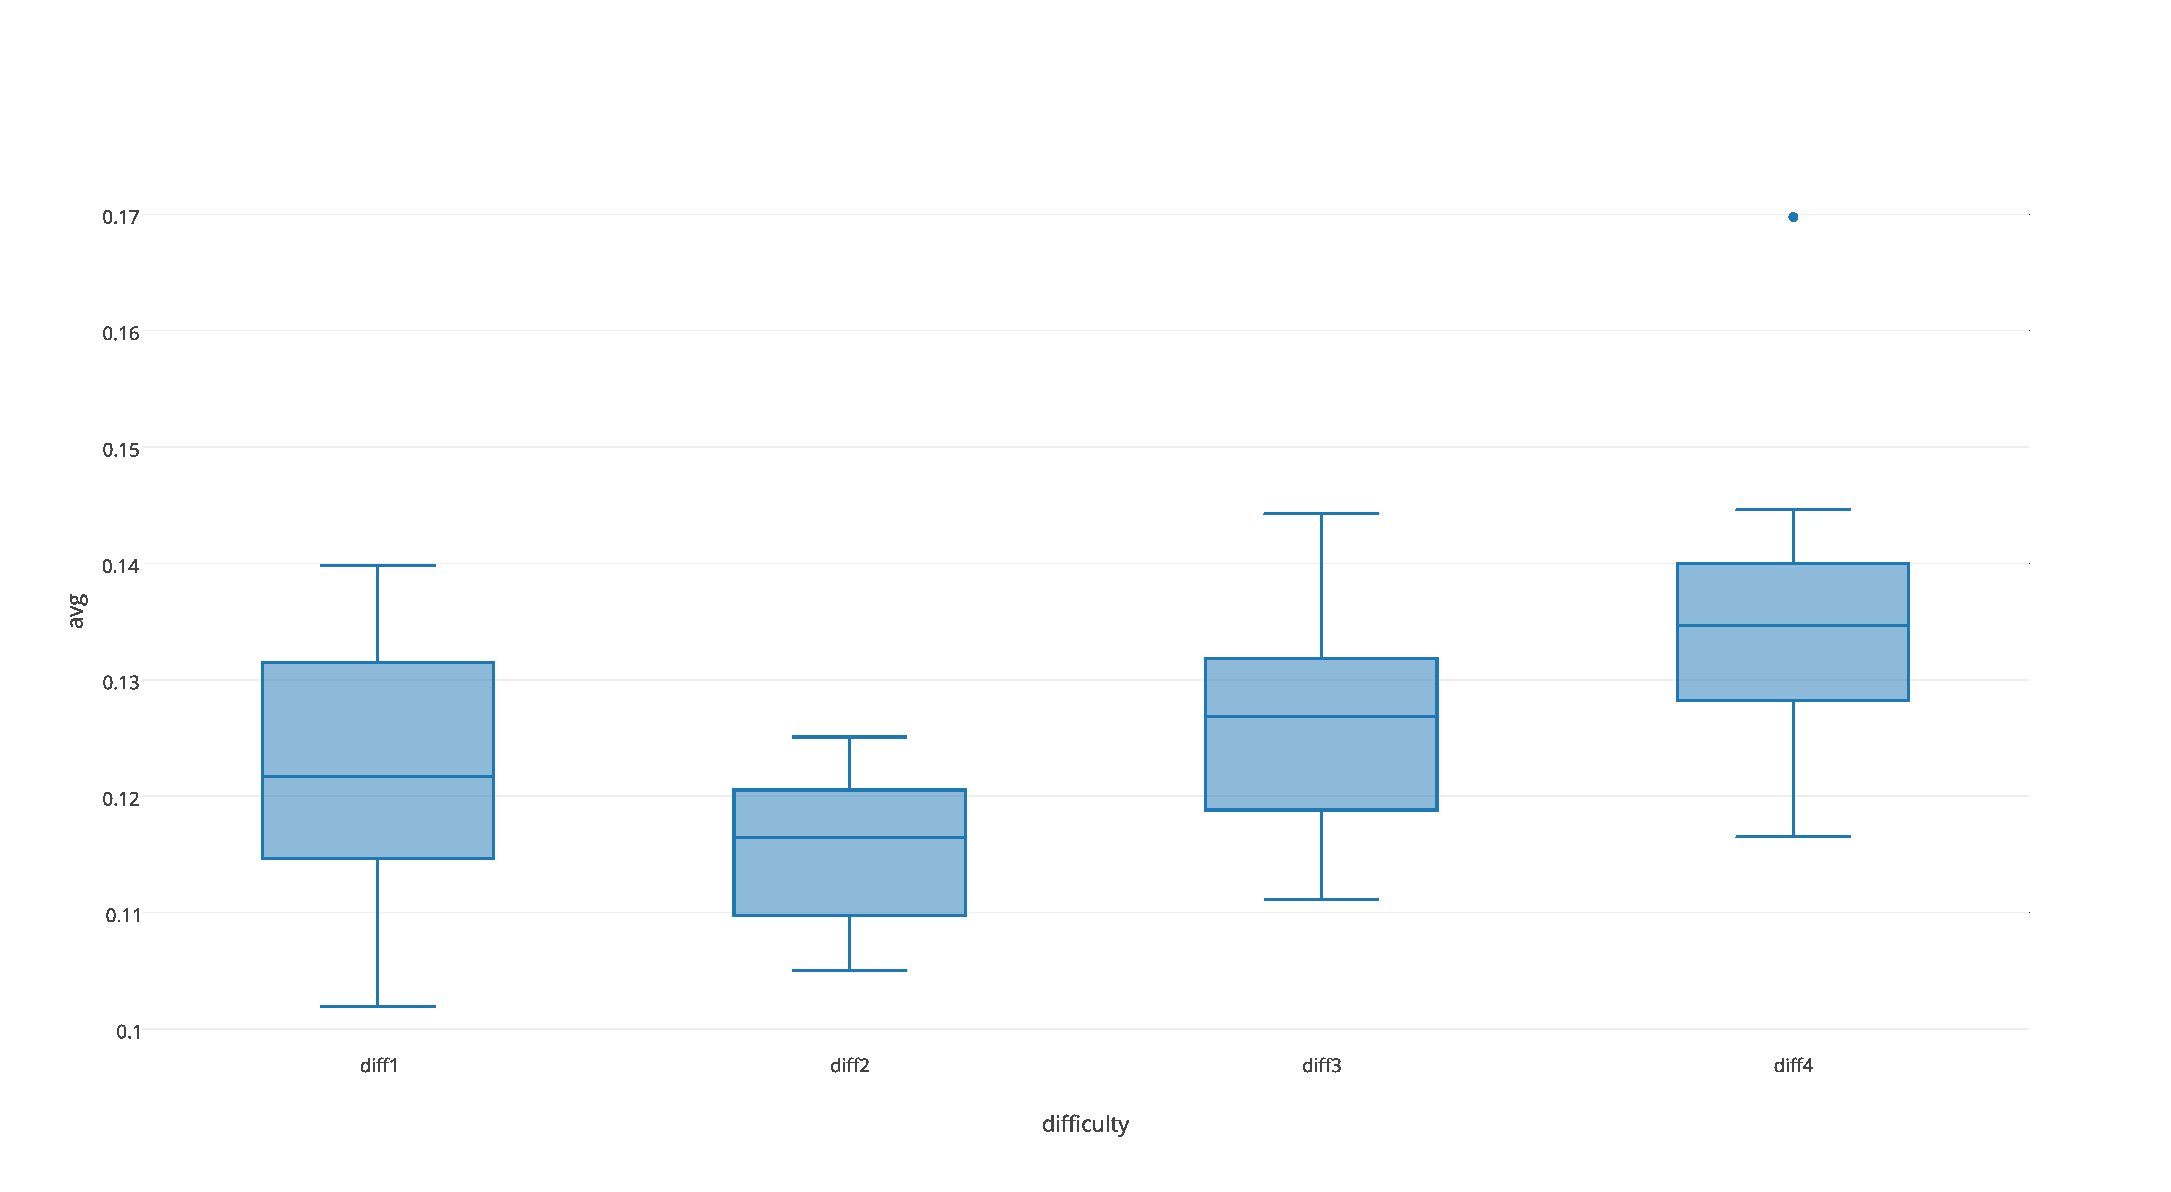
\includegraphics[width=1.6\textwidth]{avggsr.eps}
  \caption{Average GSR.}
\end{figure}

\begin{figure}[H]
  \centering
 	\hspace*{-.3\textwidth}   
 	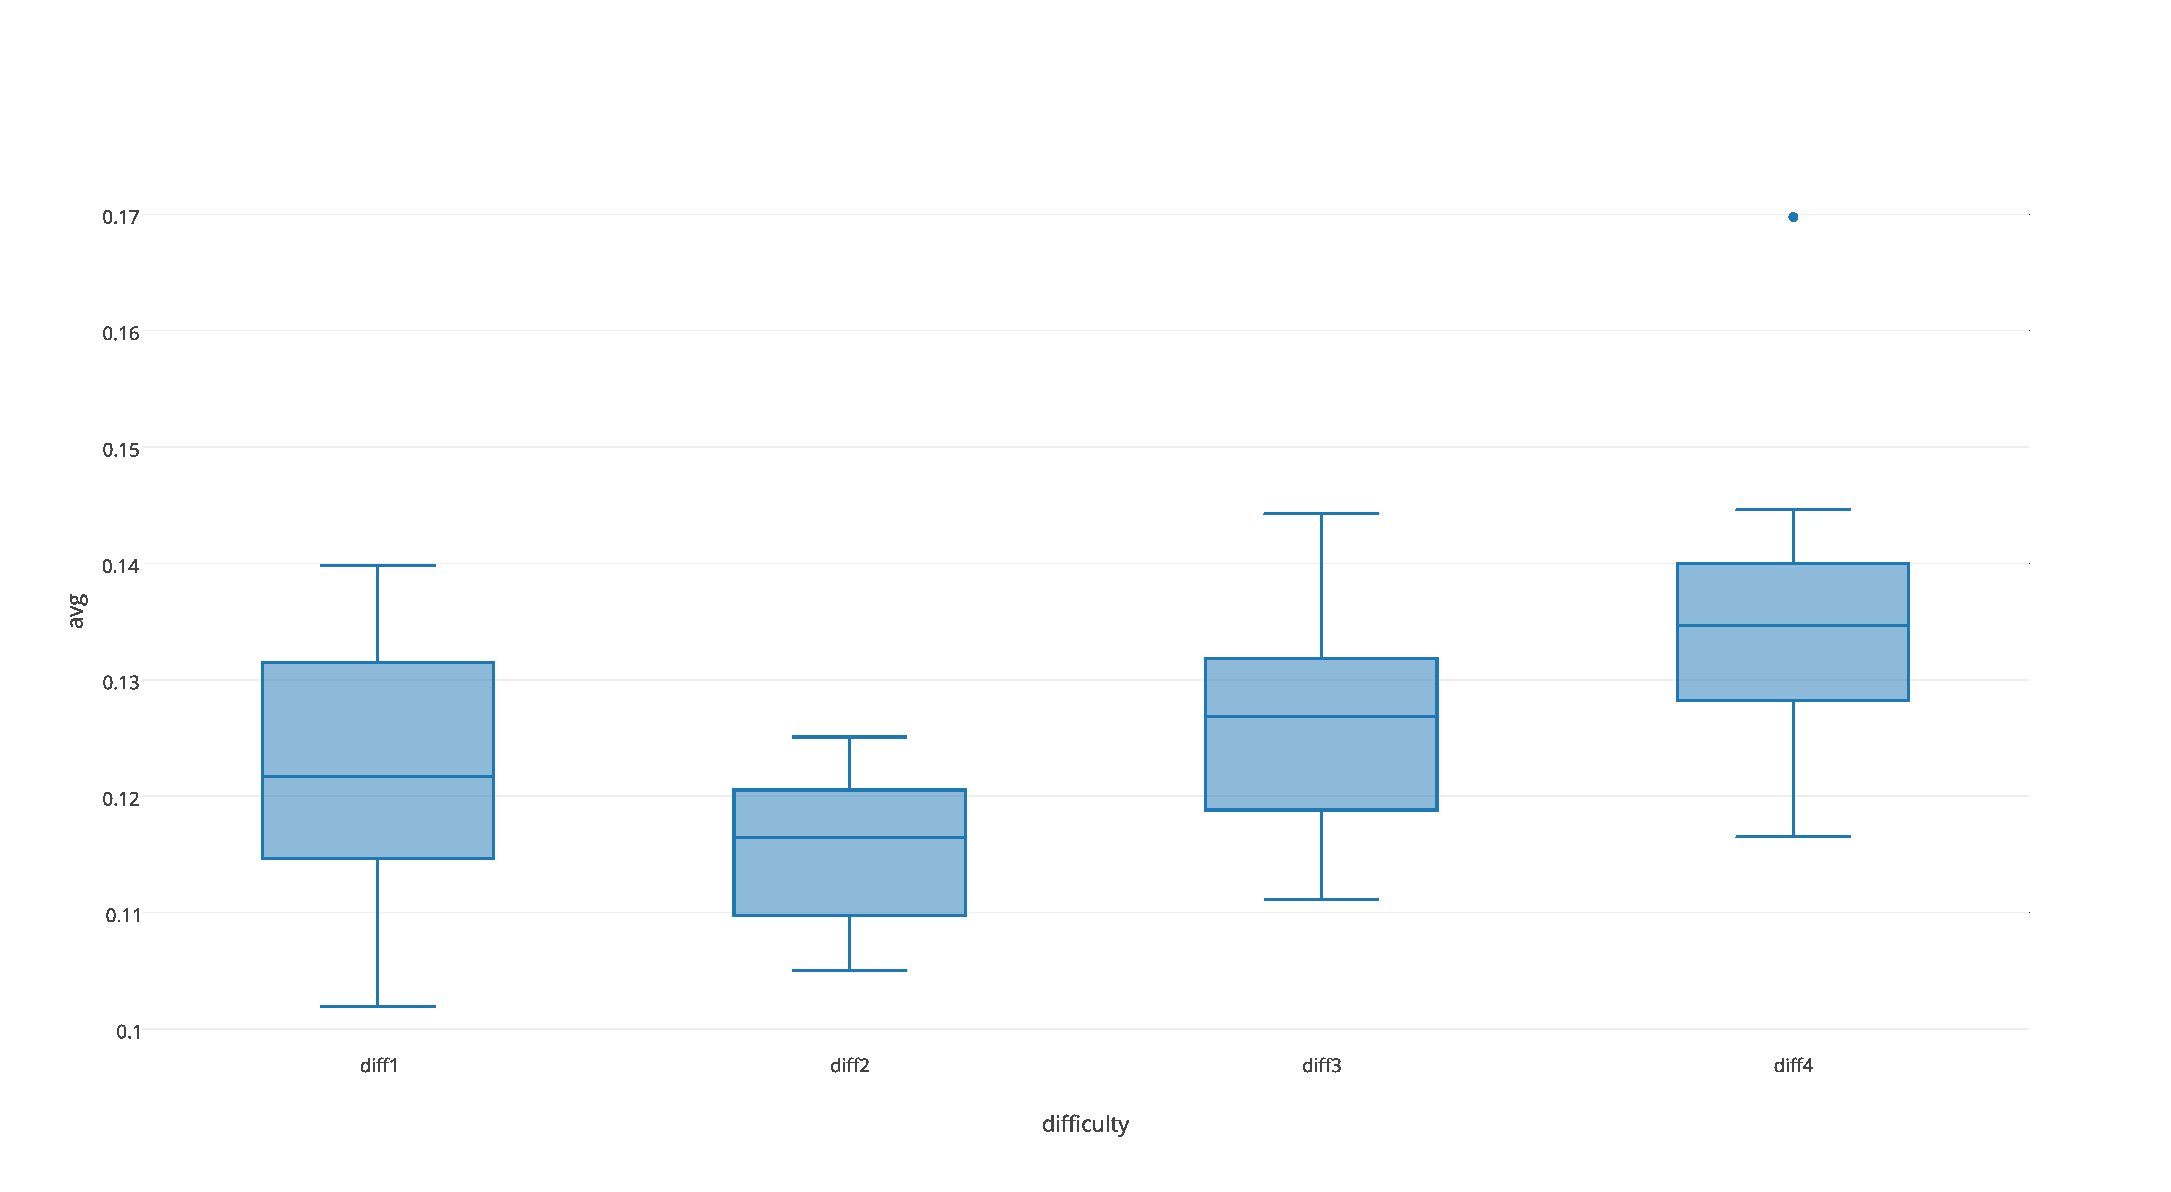
\includegraphics[width=1.6\textwidth]{avggsr.eps}
  \caption{Standard deviation.}
\end{figure}

\begin{figure}[H]
  \centering
 	\hspace*{-.3\textwidth}   
 	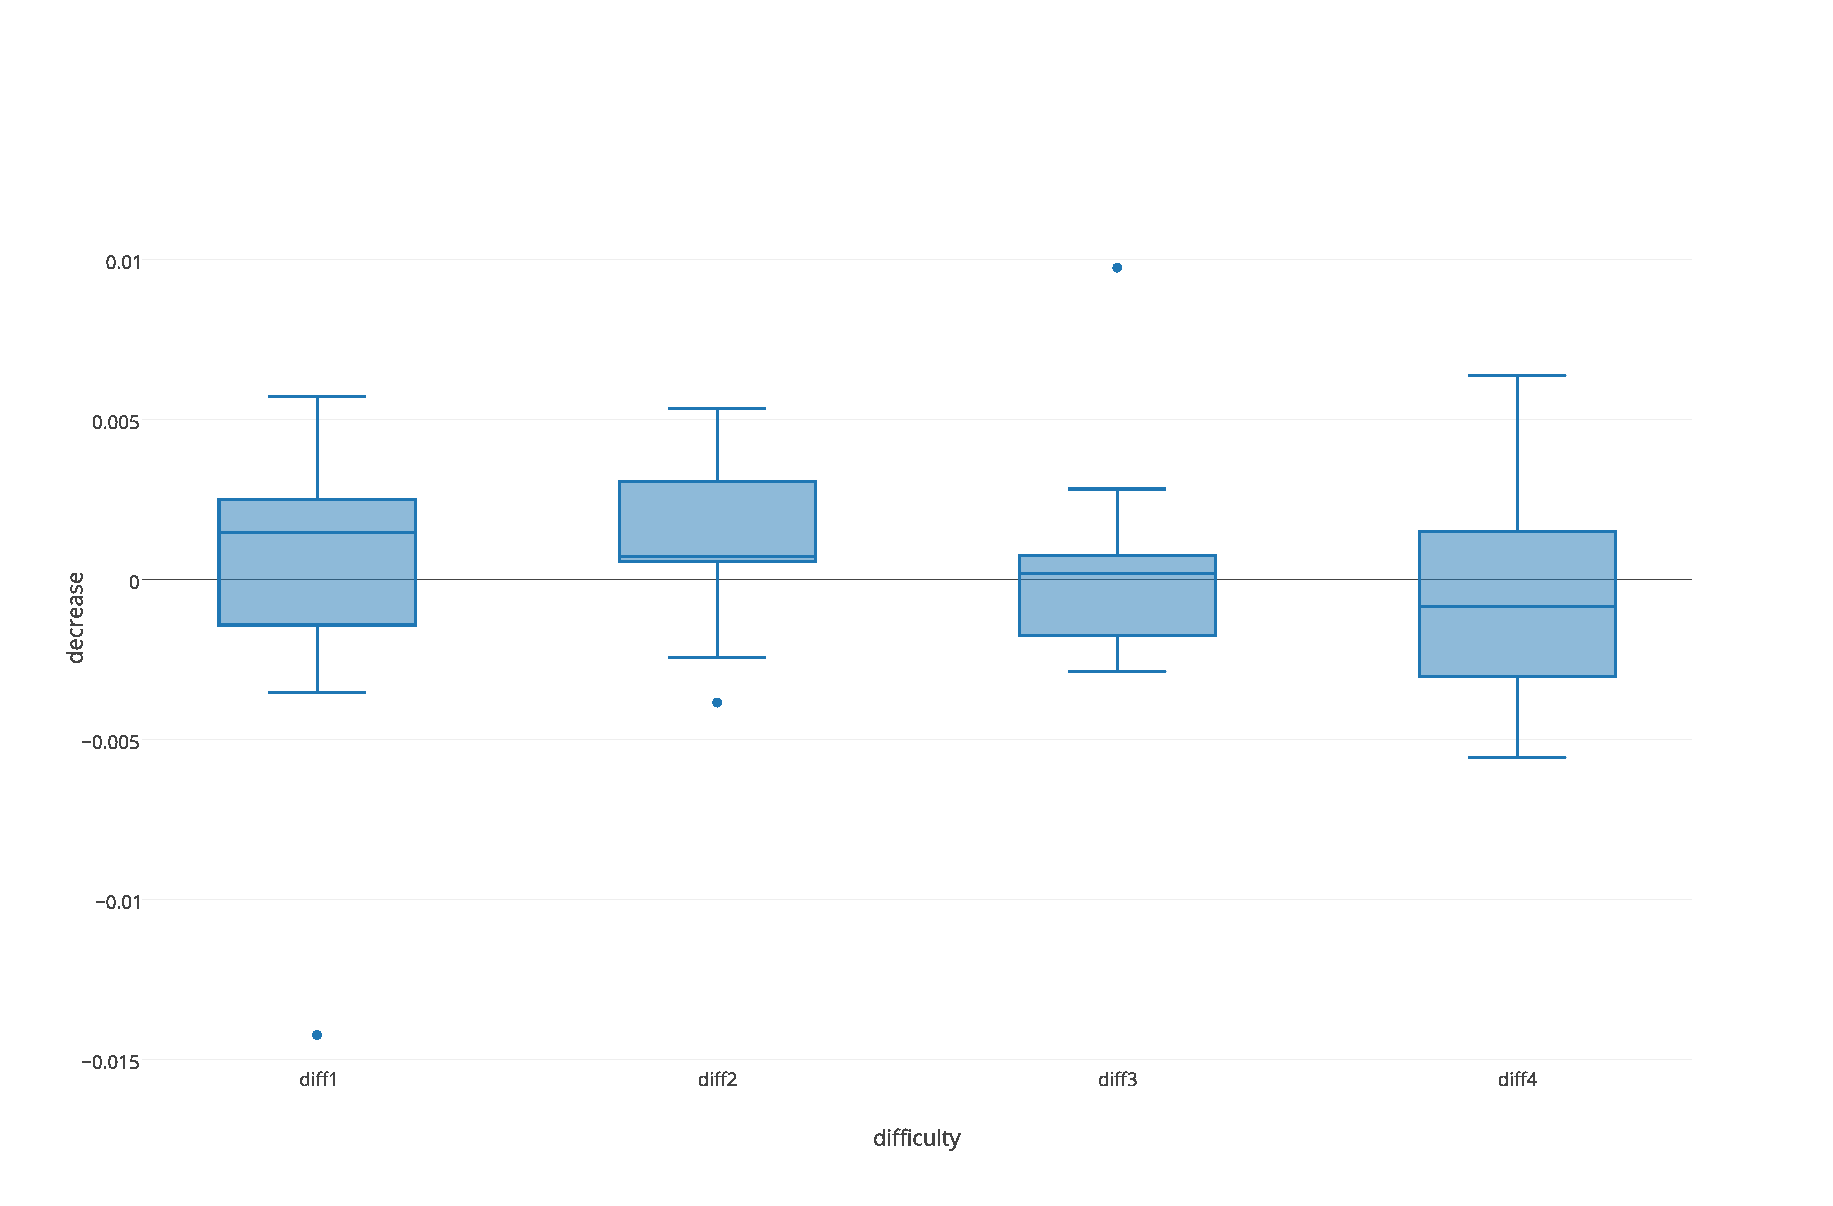
\includegraphics[width=1.6\textwidth]{decgsr.eps}
  \caption{Decrease in GSR over task.}
\end{figure}

\begin{figure}[H]
  \centering
 	\hspace*{-.3\textwidth}   
 	\includegraphics[width=1.6\textwidth]{peak.eps}
  \caption{Peak count with various tresholds.}
\end{figure}


% -- Bibliography
\bibliography{ref}{}
%\bibliographystyle{plain}

\end{document}
